\section{Quarkus Backend}
\setauthor{Oliver Sugic}

\subsection{Datenmodell}

Bevor mit der Implementierung begonnen hatte, musste zuerst eine passendes Datenmodell entworfen werden, die für Anwendung passt. Ein erster Entwurf wurde daher konzipiert, um die Datenstruktur zu definieren.

\begin{figure}[H]
    \centering
    \includegraphics[width=0.8\textwidth]{pics/Datenmodell.png}
    \caption{Erstes Entwurf des Datenmodells}
    \label{fig:datenmodell}
\end{figure}

Es gibt 5 Entitäten:

\begin{itemize}
    \item Member: Ist eine teilnehmender Schüler der Reise
    \item Event: Ist die Reise selbst
    \item Topic: Ist ein Thema, das in der Reise behandelt wird beispielsweise die Stadt Rom
    \item Activity : Ist eine Aktivität, die in der Reise stattfindet beispielsweise ein Besuch im Colosseum
    \item Staff: Ist eine Begleitperson der Reise beispielsweise ein Lehrer
\end{itemize}


Doch nach dem Entwurf musste das Datenmodell nochmal neu überarbeitet werden, da die Entität "`Staff" überflüssig war. 


\begin{figure}[H]
    \centering
    \includegraphics[width=0.8\textwidth]{pics/datenmodell_1.png}
    \caption{Überarbeiteter Entwurf des Datenmodell}
    \label{fig:datenmodell_Second}
\end{figure}

Hier sieht man das überarbeitete Datenmodell. Es gibt nun nur noch 4 Entitäten:

\begin{itemize}
    \item Person: Ist eine Teilnehmer Schüler der Reise
    \item Event: Ist die Reise selbst
    \item Topic: Ist ein Thema, das in der Reise behandelt wird beispielsweise die Stadt Rom
    \item Activity: Ist eine Aktivität, die in der Reise stattfindet beispielsweise ein Besuch im Colosseum
\end{itemize}

Die "`Staff" Entität wurde entfernt und zum Enum "`Role" hinzugefügt. Es gibt 3 verschiedene Rollen für eine teilnehmende Person:

\begin{itemize}
    \item IN-Charge: die verantwortliche Person der Reisen
    \item Staff: die Personen, die die Reise begleiten und bei der Organisation helfen
    \item Member: die Schüler der Reise 
\end{itemize}

Während der Implementierung wurde das Datenmodell nochmal überarbeitet, da man wenige Attribute hinzugefügt hat, die während der Implementierung benötigt wurden. 

\begin{figure}[H]
    \centering
    \includegraphics[width=0.6\textwidth]{pics/datenmodell_2.png}
    \caption{Endgültiger Entwurf des Datenmodell}
    \label{fig:datenmodell_Last}
\end{figure}

Hier ist das endgültige Datenmodell zu sehen. Die wohl wichtigste Änderung ist das Attribut "`currentEvent", was die aktuelle Reise der Person angibt. Somit konnte in der neuen Anzeige\ref{lst:new_view} die aktuelle Reise angezeigt werden. Auch für das Dashboard \ref{lst:dashboard} wurde das Attribut benötigt, um die Reise zu wählen, welche in der Anzeige\ref{lst:new_view} angezeigt werden soll.


\subsection{Quarkus}

Für die Verwaltung der Daten wurde ein Backend entwickelt und implementiert. Es wurde mit den Quarkus Framework geschrieben.


Quarkus ist ein Java-Framework, welches von der Firma RedHat entwickelt wurde. Es ermöglicht durch Verarbeitung der Anwendungscode, während des Kompilierens und der Ausführung, eine schnellere Startzeit und eine geringere Speicherauslastung. Dies wirkt sich positiv auf die Java Virtual Maschine aus. \cite{Thomas}

\begin{figure}[H]
    \centering
    \includegraphics[width=1\textwidth]{pics/quarkus_Memory.png}
    \caption{Quarkus Speicher Verbrauch \cite{Quarkus} }
    \label{fig:quarkus_memory}
\end{figure}


Wie man in der überliegenden Abbildung \ref{fig:quarkus_memory} sehen kann, ist der gebrauchte Speicher von einer nativen kompilierten Quarkus Anwendung, egal ob REST mit CRUD Funktionalität oder ohne. Dies war einer der Gründe warum man für dieses Projekt Quarkus gewählt hat. Außerdem hat die Erfahrung mit dem Framework auch eine tragende Rolle gespielt.

\newpage

\subsection{Implementierung des Backend}

Da nun das Datenmodell und das Framework festgelegt waren, konnte mit der Implementierung begonnen werden. Das backend sollte die Schnittstelle zum Frontend sein, aber auch die Datenbank verwalten.


\section{Angular Frontend}
\setauthor{Oliver Sugic}
Für die graphische Oberfläche wurden verschiedene Ideen und Konzepte ausprobiert, um die Benutzbarkeit für die Lernenden und Lehrenden zu optimieren.
Im Laufe des Kapitels wird erläutert, welche Versionen der Anzeige es gab und welche Versionen sich als sinnvoll erwiesen haben.

\subsection{Version 1: Visualisierung mit Karten}
\setauthor{Oliver Sugic}
Am Anfang wurden Überlegungen angestellt, wie man die Lernenden als auch die Lehrenden am besten in nicht vertrautes Gebiet führen kann.
Da die meisten Person mit Kartenservices, wie beispielsweise Google Maps oder ähnlichen Dienstleistungen, vertraut sind, wurde eine Karte implementiert.
Es gibt viele verschiedene Anbieter von Kartenservices, die in Betracht gezogen wurde. 
Da Google Maps eines der bekanntesten Anbieter, wurde auf die Google Maps Api gesetzt. 
Doch im Laufe der Recherche ist klar geworden, dass die Google Maps Api nicht die beste Lösung für dieses Projekt ist  aus folgenden Gründen: 
\begin{itemize}
    \item Die Google Maps Api läuft über die Google Cloud und ist daher kostenpflichtig
    \item Google Maps Api ist nicht open-source
    \item Google Maps Api ist nicht einfach zu anzupassen an die Bedürfnisse des Projektes 
\end{itemize}\cite{Ashraf}

\subsubsection{Leaflet Karten}
Auf der Suche nach weiteren Alternativen, verwies mich mein Klassenkollege Herr Pavelescu auf die Open-Source Kartenlösung Leaflet.

Leaflet ist eine JavaScript Libary, die es ermöglicht, Karten in Webanwendungen zu integrieren. \cite{Agafonkin} 

\newpage


\begin{lstlisting}[numbers=left,language=HTML,caption={Implementierung einer Karte mit Leaflet},label={lst:leafletmap}]{}
    <style>
    #map { height: 1000px; }
    </style>
    </head>
    <body>
     <link rel="stylesheet" href="https://unpkg.com/leaflet@1.9.3/dist/leaflet.css"
         integrity="sha256-kLaT2GOSpHechhsozzB+flnD+zUyjE2LlfWPgU04xyI="
         crossorigin=""/>
    
     <script src="https://unpkg.com/leaflet@1.9.3/dist/leaflet.js"
         integrity="sha256-WBkoXOwTeyKclOHuWtc+i2uENFpDZ9YPdf5Hf+D7ewM="
         crossorigin=""></script>
    
     <div id="map"></div>
      <script>
    var map = L.map('map').setView([48.2684159, 14.2517532], 20);
    L.tileLayer('https://tile.openstreetmap.org/{z}/{x}/{y}.png', {
        maxZoom: 19,
        attribution: '&copy; <a href="http://www.openstreetmap.org/copyright">OpenStreetMap</a>'
    }).addTo(map);
    </script> 
\end{lstlisting}

\begin{figure}[h]
\centering
\includegraphics[scale=0.2]{pics/leafletmap.png}
\caption{Ergebnis der Implementierung mit Leaflet}
\end{figure}


\subsection{Version 2: Leaflet Karte mit Routing}
\setauthor{Oliver Sugic}
Nach dem ersten Prototypen mit Leaflet, wurde die Idee weiter verfolgt, um die Benutzerfreundlichkeit für die Teilnehmenden zu verbessern. 
Eine Route vom eigenen Standort zur nächsten Aktivität wurde implementiert. 
Um die Routen anzeigen zu können, wurde die Leaflet Routing Machine verwendet. 
Hierfür wird das Plugin Leaflet Routing Machine verwendet, das ebenfalls vom Leaflet zur Verfügung gestellt wird. Mit dieser Erweiterung Können Routen zwischen zwei Punkten auf der Karte berechnet werden und angezeigt werden. Ebenfalls können die Wegpunkte einfach geändert werden.\cite{Liedman2015}  

\begin{lstlisting}[numbers=left,language=HTML,caption={Implementierung einer Karte mit Leaflet Routing Engine},
    label={lst:leafletmap}]
<head>
    <title>Leaflet Karte</title>
    <style>
        #map {
            height: 1500px;
        }
    </style>
</head>

<body>
    <link rel="stylesheet" href="https://unpkg.com/leaflet@1.9.3/dist/leaflet.css"
        integrity="sha256-kLaT2GOSpHechhsozzB+flnD+zUyjE2LlfWPgU04xyI=" crossorigin="" />

    <script src="https://unpkg.com/leaflet@1.9.3/dist/leaflet.js"
        integrity="sha256-WBkoXOwTeyKclOHuWtc+i2uENFpDZ9YPdf5Hf+D7ewM=" crossorigin="">
        </script>
    <link rel="stylesheet" href="https://unpkg.com/leaflet@1.2.0/dist/leaflet.css" />
    <link rel="stylesheet" 
    href="https://unpkg.com/leaflet-routing-machine@latest/dist/leaflet-routing-machine.css" />
    <script 
    src="https://unpkg.com/leaflet@1.2.0/dist/leaflet.js"></script>
    <script src="https://unpkg.com/leaflet-routing-machine@latest/dist/leaflet-routing-machine.js"></script>

    <div id="map"></div>
    <script>
        var map = L.map('map').setView([48.2684159, 14.2517532], 15);
        L.tileLayer('https://tile.openstreetmap.org/{z}/{x}/{y}.png', {
            maxZoom: 19,
            attribution: '&copy; <a href="http://www.openstreetmap.org/copyright">OpenStreetMap</a>'
        }).addTo(map);
        L.Routing.control({
            waypoints: [
                L.latLng(48.2684159, 14.2517532),
                L.latLng(48.2627373, 14.2589871)
            ]
        }).addTo(map);
    </script>
</body>
\end{lstlisting}

\begin{figure}[h]
    \centering
    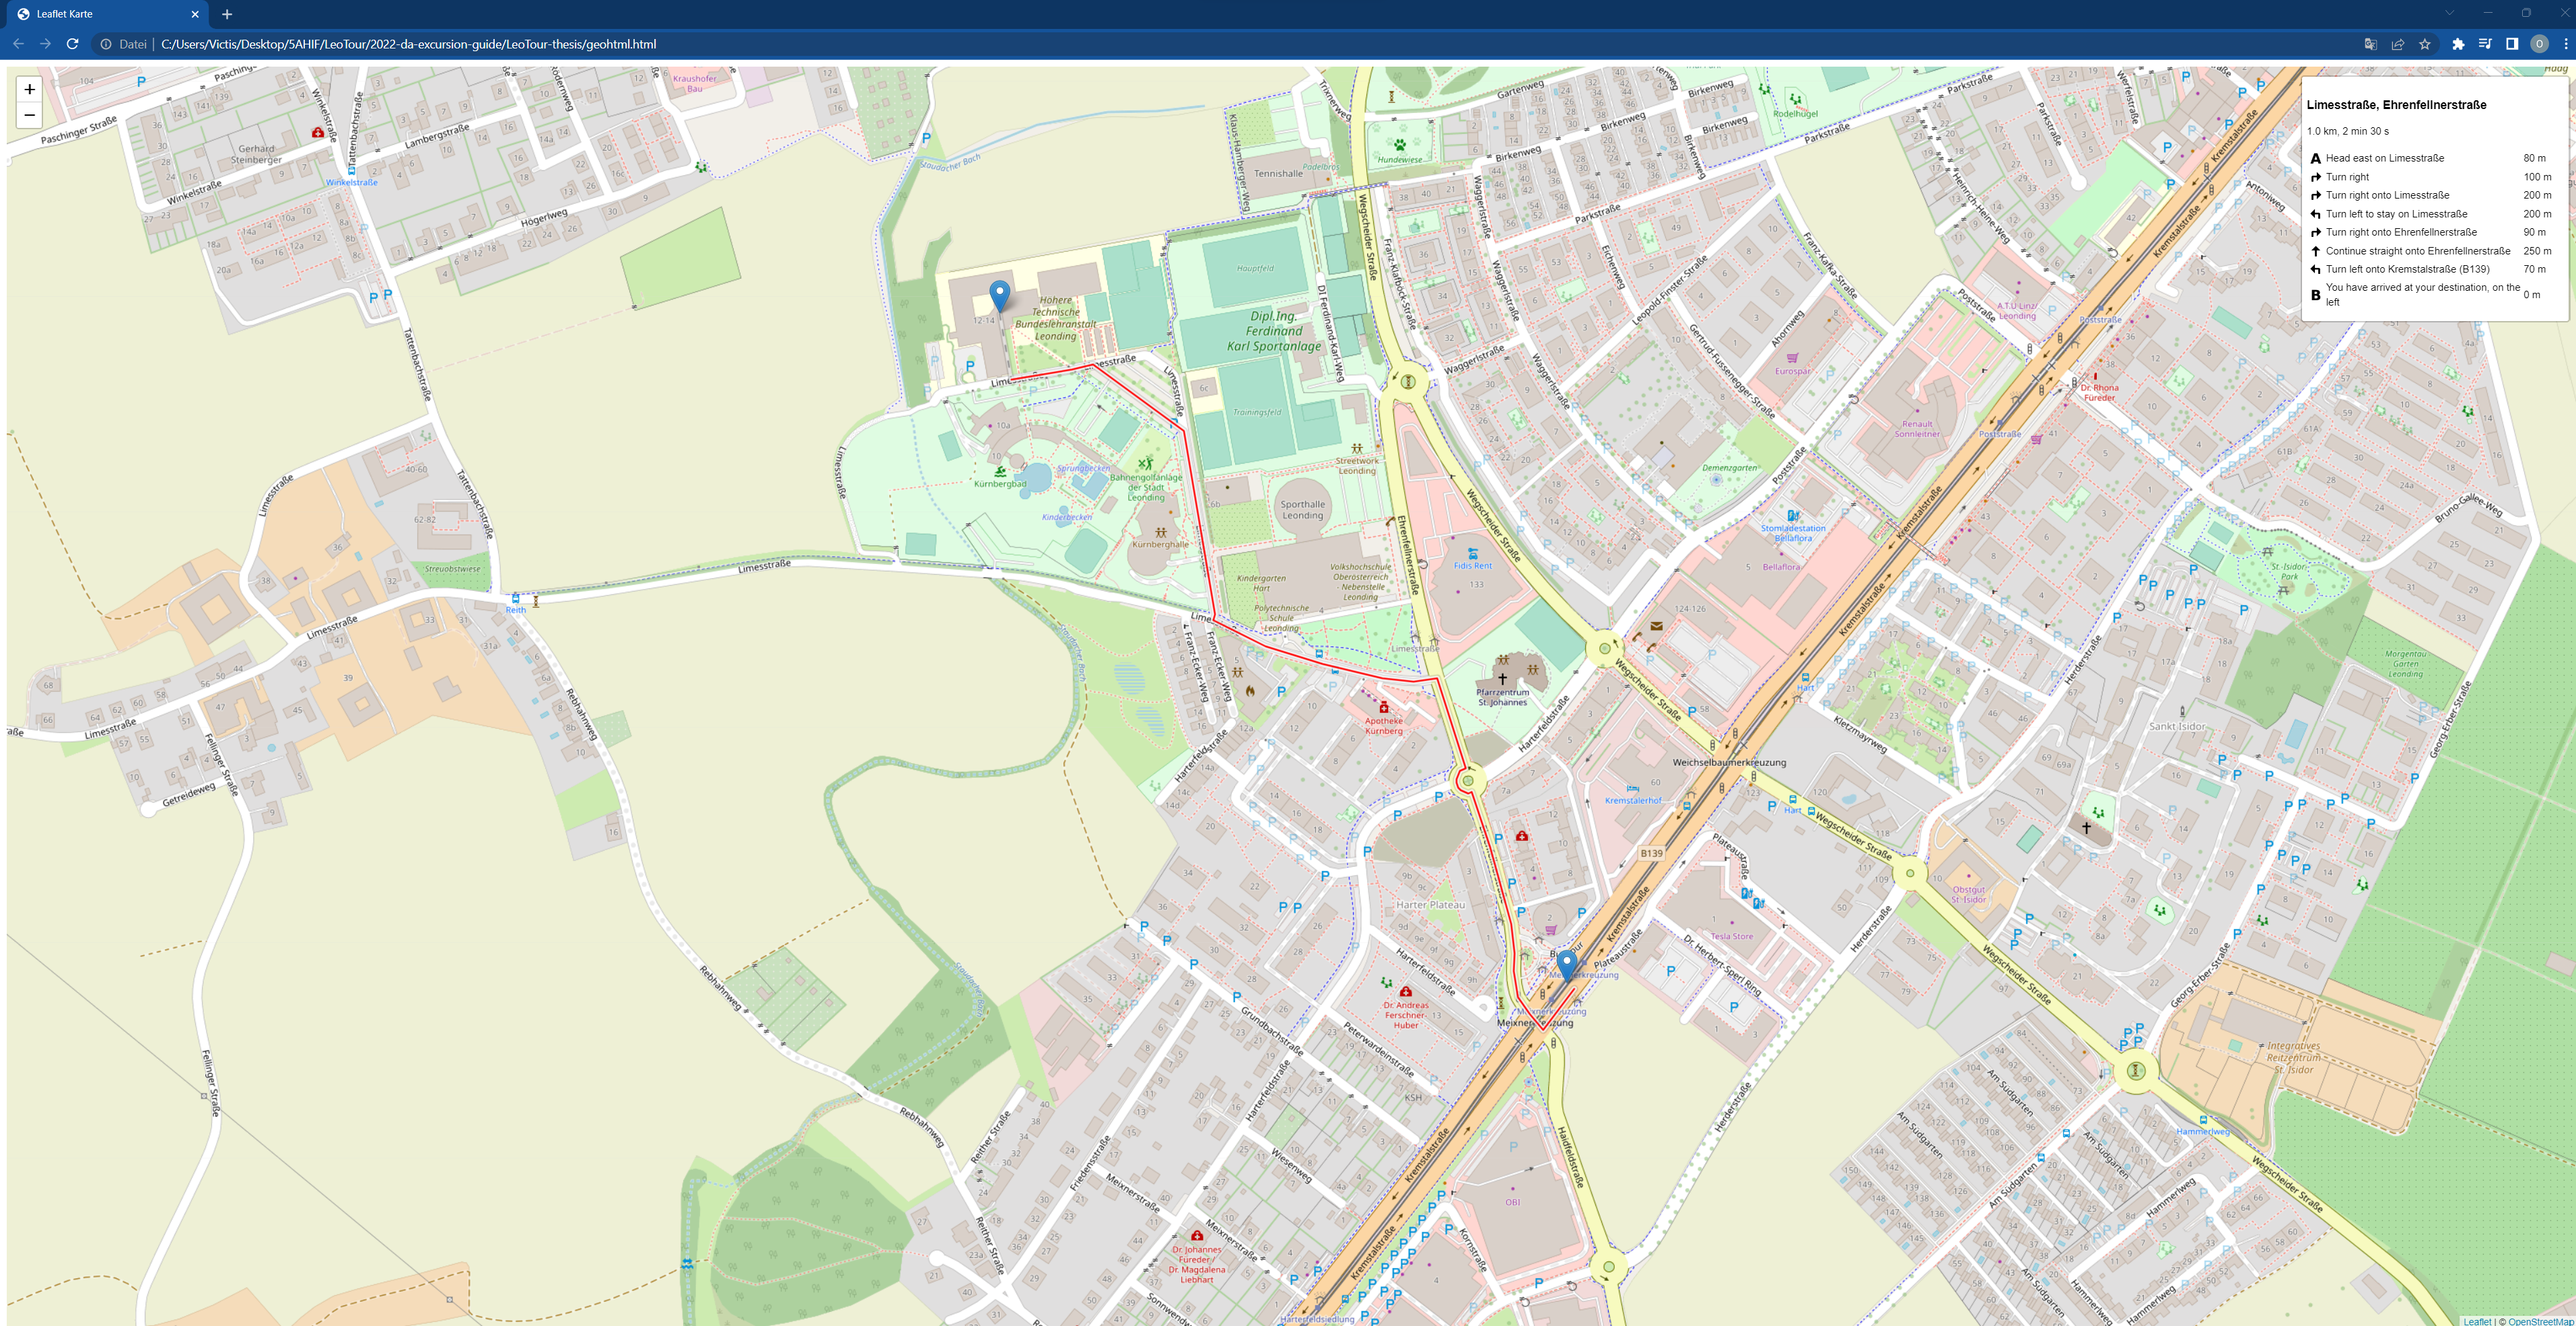
\includegraphics[scale=0.15]{pics/Leaflet_Routing.png}
    \caption{Ergebnis der Implementierung mit Leaflet Routing Machine}
\end{figure}

Allerding traten bei der Implementierung Probleme auf. Das Plugin konnte nicht die Route darstellen, was auf einen Fehler in der Implementierung zurückzuführen war.

\subsection{Version 3: Angular Geoloaction API}
\setauthor{Oliver Sugic}
Da die Implementierung mit der Leaflet Routing Machine nicht funktioniert hat, wurde versucht, mittels des Standorts des Nutzenden zur nächsten Aktivität zu navigieren. 

\section{Aktuelle Komponenten}
\setauthor{Oliver Sugic}
Derzeit besteht die Anwendung aus drei Komponenten. In diesem Kapitel werden der Aufbau und und Zusammenhänge der einzelnen Komponenten erläutert.  

\subsection{Angular Frontend}
\setauthor{Oliver Sugic}
Der schwierigste Teil der Arbeit liegt darin, eine Benutzeroberfläche zu erstellen, die einfach zu bedienen aber auch ansprechend für den Benutzer ist.
Es wurde daher auf das Angular Framework genommen, da es sehr 

\subsubsection{Schüler Sicht}

Nach dem Scheitern der Implementierung mit der Leaflet Routing Machine, wurde eine neues Design entworfen, um die Benutzerfreundlichkeit zu verbessern.
Nach vielen Überlegung wurde ein Wireframe entworfen \ref{lst:Wireframe}, welches sowohl für mobile Endgeräte geeignet ist, aber auch überschaubar für die nutzenden Personen ist.

\begin{figure}[h]
    \centering
    \includegraphics[scale=0.3]{pics/Wireframe.png}
    \caption{Entwurf der Schüleransicht }
    \label{lst:Wireframe}
\end{figure}


Der Nutzer soll in einen groben Überblick haben, welche Städte er besuchen wird. Durch eine kurze Beschreibung der Aktivität solle der Reisende einen kurzen Einblick haben, was Ihn erwarten wird. In der unteren Hälfte des Bildschirm erhält man genauere Informationen über den Treffpunkt, außerdem ist es möglich sich auf der Karte die Route anzeigen zu lassen. Es ist möglich, sich auf der standartmäßigen Karte des Endgeräts, über Google Maps oder über die OpenStreetMap zu navigieren. Der Nutzende kann für sich entscheiden, welche Karte Ihm am besten gefällt oder welche Karte Ihm am meisten vertraut ist wie in Abbildung \ref{lst:Overview} zu sehen ist.

\begin{figure}[h]
    \centering
    \includegraphics[scale=0.8]{pics/overview.png}
    \caption{Schüler Ansicht}
    \label{lst:Overview}
\end{figure}

Da den Schüler und Schülerinnen die Mitführung von elektronischen Geräten, müssen die Schüler und Schülerinnen Ihre Handys benutzen, da die Mitführung eines Handys nicht verboten ist. Somit musste die Ansichten für mobil Geräte angepasst werden. 

\subsubsection{Aktivitäten freischalten}
Um die Aktivitäten freizuschalten, kann der Lehrer über die Unlock-Activity Komponente die Aktivitäten freischalten. Es werden alle Aktivitäten angezeigt und kann durch bedienen des Buttons freigeschaltet werden oder auch wieder gesperrt werden.

\begin{figure}[h]
    \centering
    \includegraphics[scale=0.8]{pics/unlock-activity.png}
    \caption{Aktivitäten freischalten und sperren}
    \label{lst:UnlockActivity}
\end{figure}

Wieder musste auf die mobile Ansicht geachtet werden. Die Lehrer oder die Lehrerinnen haben zwar einen Laptop mit, aber da es sehr unpraktisch ist mit einem Laptop durch unbekanntes Gebiet herumzureisen, wurde die Ansicht für mobile Geräte angepasst. 

\subsubsection{Event erstellen}
Für das erstellen eines Events wurde eine eigene Komponente entworfen und entwickelt. Da eine Lehrkraft in die Reise im voraus planen muss, ist sie für den Gebrauch von Laptops angepasst worden.

Die Komponente wurde in vier Abschnitte geteilt:

\begin{itemize}
    \item Daten des Events
    \item Daten der Teilnehmer 
    \item Daten des Themas
    \item Daten der Aktivitäten
\end{itemize}

\begin{figure}[h]
    \centering
    \includegraphics[scale=0.35]{pics/create-event.png}
    \caption{Abschnitt für die Daten des Events}
    \label{lst:event}
\end{figure}

\begin{figure}[h]
    \centering
    \includegraphics[scale=0.35]{pics/add-participant.png}
    \caption{Abschnitt für die Daten der Teilnehmer}    
    \label{lst:participant}
\end{figure}

\begin{figure}[h]
    \centering
    \includegraphics[scale=0.35]{pics/add-topic.png}
    \caption{Abschnitt für die Daten des Themas}
    \label{lst:topic}
\end{figure}

\begin{figure}[h]
    \centering
    \includegraphics[scale=0.35]{pics/add-activites.png}
    \caption{Abschnitt für die Daten der Aktivitäten}
    \label{lst:activity}
\end{figure}

\subsubsection{Überarbeitung mit Angular Material}

Allerdings waren die Entwürfe teilweise unübersichtlich und farblich nicht ansprechend. Schlussendlich wurden alle Angular Komponenten mit Angular Material überarbeitet. Durch das hinzufügen des Angular Material Frameworks, wurde die Benutzeroberfläche ansprechender und übersichtlicher.

Mit den Möglichkeiten des Angular Material Framework wurde die Benutzeroberfläche überarbeitet.

\begin{figure}[h]
    \centering
    \includegraphics[scale=0.85]{pics/new_view.png}
    \caption{Neue Oberfläche für die Schüleransicht}
    \label{lst:new_view}
\end{figure}


\newpage
Im Vergleich ist die Abbildung \ref{lst:new_view} im Vergleich mit der alten Version \ref{lst:Overview} viel ansprechender. Durch die Verwendung eines Material Cards hat der Text des ausgewählten Themas eine bessere Lesbarkeit und wird auch besser herausgehoben. Durch das Trennen der zwei Abschnitte mit Hilfe von Material Divider wird ein klare Trennung zwischen den beiden Abschnitten erreicht. Ebenso wurde die Buttons für die Navigation auf der Karte in Material Buttons umgewandelt.
\newpage
Ebenso wurde das Design für das Freischalten der Aktivitäten überarbeitet.

\begin{figure}[h]
    \centering
    \includegraphics[scale=0.85]{pics/new_unlock_activity.png}
    \caption{Neue Oberfläche für die Schüleransicht}
    \label{lst:new_unlock_activity}
\end{figure}
Im Vergleich zur alten Version \ref{lst:UnlockActivity} ist die neue Version \ref{lst:new_unlock_activity} verbessert worden. Die Buttons wurden in Material Buttons umgewandelt und so entworfen, dass die Lehrerinnen und Lehrer einen direkten Überblick haben, welche Aktivitäten freigeschaltet sind und welche nicht.
\newpage

Neu ist auch die Ansicht zum erstellen eines Events. Da beim Testen der alten Version festgestellte wurde, dass diese nicht die Funktionalität erfüllt, musste die Komponente neu entworfen werden. Dazu entschloss man sich für die Umsetzung, den Angular Material Stepper zu verwenden. Dieser ermöglicht es, die einzelnen Abschnitte des Events in einzelne Schritte zu unterteilen. Praktisch ist auch, das der Stepper die Möglichkeit bietet, Schritte zurückzugehen, um die Eingaben zu korrigieren. Mit Hilfe des Steppers ist das Erstellen eines Events einfacher und besser im Vergleich zur Vorgänger Version.


\begin{itemize}
    \item Daten des Events
    \begin{figure}[h]
        \centering
        \includegraphics[scale=0.27]{pics/new_create_1.png}
        \caption{Neue Oberfläche für die Eingabe der Daten des Events}
        \label{lst:new_create_event_1}
    \end{figure}
    \item Daten der Personen
    \begin{figure}[h]
        \centering
        \includegraphics[scale=0.27]{pics/new_create_2.png}
        \caption{Neue Oberfläche für die Eingabe der Daten der Personen}
        \label{lst:new_create_event_2}
    \end{figure}
    

    \newpage
    \item Daten der Themen
    \begin{figure}[h]
        \centering
        \includegraphics[scale=0.27]{pics/new_create_3.png}
        \caption{Neue Oberfläche für die Eingabe der Daten der Themen}
        \label{lst:new_create_event_3}
    \end{figure} 
    Die Oberfläche wurde so gelöst, dass die Lehrerinnen und Lehrer bei der Eingabe der Daten ein direkte Übersicht haben, welche Themen angelegt wurden. Beim Anklicken eines Themas werden die bereits angelegten Aktivitäten angezeigt. Beim Anklicken des Buttons "`Add Activity`" wird ein Dialog geöffnet, in dem die Daten für eine neue Aktivität eingegeben werden können.  

    \item Daten der Aktivitäten
    \begin{figure}[h]
        \centering
        \includegraphics[scale=0.27]{pics/new_create_3_1.png}
        \caption{Neue Oberfläche für die Eingabe der Daten der Aktivitäten}
        \label{lst:new_create_event_3_1}
    \end{figure}    
\end{itemize}

Nach dem die Komponente für das Anlegen der Events nun fertig war, stellte man fest, das man keine Übersicht hat über die schon geplanten Reisen. Außerdem musste man einen Weg finden, dass die Lehrerinnen und Lehrer die richtige Reise auswählen können.

\newpage
Nach mehreren Überlegungen, entschloss man sich für die Erstellung einer Komponente. Die sollte als Übersicht oder auch als "`Dashboard`" dienen. Wie sie implementiert werden sollte, war nicht ganz klar. Hierbei gab es verschiedene Möglichkeiten, welche man in Betracht gezogen worden sind:


\begin{itemize}
    \item Anzeige der Events an die zugewiesen Schülerinnen und Schülern

    Hier war die Überlegung, dass die Lehrerinnen und Lehrer eine Reise auswählen und diese ihrer Klasse zuweisen. Die Schülerinnen und Schüler der jeweiligen Klasse können sich dann die Reise sehen. Allerdings wurde die Idee verworfen, da im Laufe der Entwicklung mit dem Keycloak Probleme entstanden, die im Kapitel \ref{sec:keycloak} beschrieben werden.

    \item Anzeige des Events an alle Personen 

    Nach dem gescheiterten Versuch mit dem Keycloak, wurde eine neue Idee umgesetzt. Lehrerinnen und Lehrer müssen die Schulexkursion oft mehrere Monate im voraus planen. Jeder kann sich die Reise ansehen, die gerade oder als nächstes stattfindet.
\end{itemize}

\begin{figure}[h]
    \centering
    \includegraphics[scale=0.2]{pics/dashboard.png}
    \caption{Dashboard für die Lehrerinnen und Lehrer}
    \label{lst:dashboard}
\end{figure}    

Hier werden die Reisen aufgelistet werden und die Lehrerinnen und Lehrer haben die Möglichkeit haben, ihre geplante Reise auszuwählen.
Am oberen Rand befindet sich ein Button "`Neu Reise anlegen`" mit dem man sich zum Erstellen von Reisen navigieren kann. Nachdem man eine Reise angeklickt hat, kann man sich Informationen über Reise einholen. Ebenso kann man zum Freischalten der Aktivitäten navigieren, hierfür gibt es auch einen Button "`Aktivitäten freischalten`". Falls die Lehrerin oder der Lehrer nicht sicher sind, ob zu viele Informationen über die Reise vorhanden sind, können sie via den Button "`Reise in der Schüleransicht anzeigen`" die Reise zu Überprüfung in der Schüleransicht nachsehen.

\newpage


\section{Keycloak}\label{sec:keycloak}
\setauthor{Oliver Sugic}


Um die Anwendung zu schützen, braucht es einen Authentifizierungsserver. Dieser ist für die Anwendung sehr wichtig, da die Schülerinnen und Schüler nur die Reise sehen können, die ihnen zugewiesen wurde. Außerdem können nur Lehrerinnen und Lehrer Reisen erstellen und bearbeiten. Um sich von große Firmen loszulösen wie beispielsweise von Google. Sollte daher bei einem Daten Leak von Google keine Daten von Schülerinnen und Schülern betroffen sein. Wurde daher Keycloak als Authentifizierungsserver gewählt. Keycloak ist ein Open-Source-Software-Produkt, das als Authentifizierungsserver und Identityprovider dient. Außerdem bietet Keycloak den Vorteil, das nicht nur die Autorisierung übernimmt sondern auch die Authentisierung der Benutzer. Ebenfalls kann er mit Active-Directory-Servern authentifizieren, was für die Anwendung sehr praktisch ist, da die HTBLA Leonding bereits so ein System besitzt.  \cite{Keycloak} 


Zwar wurde Anfang auf ein eigene Keycloak gesetzt, doch schnell wurde klar, das es einfach wäre, den Keycloak zu nehmen der von der Schule bereit gestellt wird, um sich mit den Schüler Login Daten anzumelden. 


Dieser wurde im Angular Frontend eingebunden. Somit wurde eine neue Komponente erstellt, welche den Zweck hat, den Login und Logout zu ermöglichen. Außerdem wurde überprüft ob der Benutzer ein als Schülerin oder Schüler angemeldet ist. Falls ja, wird die Komponente für die Schülerin oder den Schüler angezeigt. Falls nein, wird die Komponente für die Lehrerinnen und Lehrer angezeigt.
Im folgenden Code sieht man die Implementierung des Keycloak in Angular.

\begin{lstlisting}[numbers=left,language=typescript,caption={Implementierung im Angular},label={lst:keycloak_angular}]{}
ngOnInit() {
    this.oidcSecurityService
        .checkAuth()
        .subscribe(({isAuthenticated, userData, accessToken, idToken}) => {
        this.userData = userData;
        });
    if (this.userData.preferred_username.indexOf('.') > -1 || this.userData.preferred_username == "if180157") {
        this.isTeacher = true
    } else {
        this.isStudent = true;
    }
}
login() {
this.oidcSecurityService
    .authorizeWithPopUp()
    .subscribe(({isAuthenticated, userData, accessToken, errorMessage}) => {
    this.userData = userData;
    });
this.oidcSecurityService.authorize();
}
logout() {
this.oidcSecurityService
    .logoff()
    .subscribe((result) => console.log(result));
}
\end{lstlisting}

Nach dem allerdings diese Funktion beim Deployment getestet wurde, funktionierte der Redirect auf die eigentliche Applikation nicht mehr.

\begin{figure}[h]
    \centering
    \includegraphics[scale=0.3]{pics/keycloak.png}
    \caption{Fehlschlagender Redirect nach dem Login}
    \label{lst:keylcoak_login}
\end{figure} 

Aufgrund dessen wurde der Keycloak aus dem Projekt entfernt und eine funktionierende Anwendung zu gewährleisten.  

\newpage

\section{Deployment}
\setauthor{Oliver Sugic}

Deployment ist die Bereitstellung von Software. Es umfasst dabei Prozesse, die automatisiert werden wie die Installation, Konfiguration und weiteren auf dem Server. \cite{Deployment}


Deployment war daher für das Projekt ein wichtiger Bestandteil. Die teilnehmenden Personen müssen auch auf die Website zugreifen können, um dann die Funktionalität der Anwendung nutzen zu können. Wo die Anwendung bereitgestellt wird, gab es zwei Optionen:

\begin{itemize}
    \item LeoCloud
    \item Oracle VM
\end{itemize}

Nach nicht allzu langer Überlegungen nahmen wir die LeoCloud, welche von der Schule bereit gestellt wurde, wo die Schüler ihre Anwendung deployen können. Die Oracle VM schlossen wir aus, da sie viel zu wenig Leistung hat und die Anwendung nicht richtig laufen würde.

\newpage

Mittels Gihtub-Actions konnten wir dann die sowohl das Backend, Frontend und die Datenbank in GitHub Packages speichern. Die Github Actions sehen folgendermaßen aus:

\begin{lstlisting}[numbers=left,caption={Github Actions für das Backend},label={lst:gh_action_Backend}]{}
name: build-image-backend
on:
    push:
    branches: [ main ]

env:
    REGISTRY: ghcr.io

jobs:
    build:
    name: build
    runs-on: ubuntu-latest
    steps:
        - uses: actions/checkout@v3

        - name: convert github repository name to lowercase
        run: echo "IMAGE_REPOSITORY=$(echo ${{ github.repository }} | tr '[:upper:]' '[:lower:]')" >> $GITHUB_ENV

        - name: convert github registry name to lowercase
        run: echo "IMAGE_REGISTRY=$(echo ${{ env.REGISTRY }} | tr '[:upper:]' '[:lower:]')" >> $GITHUB_ENV

        - name: Log in to the Container registry
        uses: docker/login-action@v2
        with:
            registry: ${{ env.REGISTRY }}
            username: ${{ github.actor }}
            password: ${{ github.token }}

        - name: Set up Docker Buildx
        uses: docker/setup-buildx-action@v2

        - name: Build and push
        uses: docker/build-push-action@v4
        with:
            context: "{{defaultContext}}:backend"
            file: ./src/main/docker/Dockerfile.jvm
            push: true
            tags: ${{ env.REGISTRY }}/${{ env.IMAGE_REPOSITORY }}-backend:latest
            cache-from: type=registry,ref=${{ env.REGISTRY }}/${{ env.IMAGE_REPOSITORY }}-backend:buildcache
            cache-to: type=registry,ref=${{ env.REGISTRY }}/${{ env.IMAGE_REPOSITORY }}-backend:buildcache,mode=max
\end{lstlisting}

\newpage

Wie man bereits erkennen kann, wird diese Action immer dann ausgeführt, wenn ein Push auf den `main` Branch gemacht wird. Außerdem wird ein Image gespeichert, welches dann zu einem Github Package hochgeladen wird. Allerdings braucht es ein Dockerfile, um überhaupt ein Image zu erstellen. Dieses sieht folgendermaßen aus:


\begin{lstlisting}[numbers=left,caption=Dockerfile für das Backend,label={lst:dockerfile_Backend}]{}
FROM registry.access.redhat.com/ubi8/openjdk-17:1.13-1.1655306439 as build

USER root

COPY mvnw /code/mvnw
COPY .mvn /code/.mvn
COPY pom.xml /code/

WORKDIR /code
RUN ./mvnw -B org.apache.maven.plugins:maven-dependency-plugin:3.1.2:go-offline
COPY ./src /code/src
RUN ./mvnw package -Dmaven.test.skip

FROM registry.access.redhat.com/ubi8/openjdk-17:1.13-1.1655306439

ENV LANG='en_US.UTF-8' LANGUAGE='en_US:en'

# We make four distinct layers so if there are application changes the library layers can be re-used
COPY --from=build --chown=185 /code/target/quarkus-app/lib/ /deployments/lib/
COPY --from=build --chown=185 /code/target/quarkus-app/*.jar /deployments/
COPY --from=build --chown=185 /code/target/quarkus-app/app/ /deployments/app/
COPY --from=build --chown=185 /code/target/quarkus-app/quarkus/ /deployments/quarkus/

EXPOSE 8080
USER 185
ENV AB_JOLOKIA_OFF=""
ENV JAVA_OPTS="-Dquarkus.http.host=0.0.0.0 -Djava.util.logging.manager=org.jboss.logmanager.LogManager"
ENV JAVA_APP_JAR="/deployments/quarkus-run.jar"
\end{lstlisting}

Nach dem nun jeweils die Packages generiert waren, konnte man sich nun auf die LeoCloud konzentrieren. Dazu braucht man ein YAML File, welches das Deployment als auch den Service zu Verfügung stellt. 
Doch was ist die Aufgabe eines Services und einem Deployment? Mit einem Deployment kann ich mehrere Pods eines Kubernetes Cluster verwalten, hingegen der Service dafür zuständig ist, dass die Pods ein Netzwerkzugriff ermöglicht wird.\cite {Kubernetes}

\newpage

Da dies nun geklärt ist, schauen wir uns nun das YAML File dazu an:

\begin{lstlisting}[numbers=left,caption=Dockerfile für das Backend,label={lst:Kuberntes_yaml_Frontend}]{}
apiVersion: apps/v1
kind: Deployment
metadata:
    name: frontend-deployment
    namespace: student-o-sugic
spec:
    replicas: 1
    selector:
    matchLabels:
        app: frontend
    template:
    metadata:
        labels:
        app: frontend
    spec:
        containers:
        - name: frontend
            image: ghcr.io/htl-leonding-project/2022-da-excursion-guide-frontend:latest
            ports:
            - containerPort: 80
            imagePullPolicy: Always
---
apiVersion: v1
kind: Service
metadata:
    name: frontend-svc
    namespace: student-o-sugic
spec:
    ports:
    - port: 80
        targetPort: 80
        protocol: TCP
        name: http
    selector:
    app: frontend
\end{lstlisting}

\newpage

Zur Überprüfung wird sich das Kubernetes Dashboard kontrolliert ob keine Fehler aufgetreten sind.

\begin{figure}
    \centering
    \includegraphics[width=0.9\textwidth]{pics/kubernetes_dashboard.png}
    \caption{Kubernetes Dashboard}
    \label{fig:Kubernetes_dashboard}
\end{figure}
\begin{figure}
    \centering
    \includegraphics[width=0.9\textwidth]{pics/kubernetes_services.png}
    \caption{Kubernetes Services}
    \label{fig:Kubernetes_dashboard_Services}
\end{figure}


\subsection{Mögliche zukünftige Erweiterungen}
\setauthor{Oliver Sugic}

Für die Zukunft könnten weiter mögliche Erweiterungen implementiert werden:

\begin{itemize}
    \item Entwicklung einer Mobile App mit Android oder Swift
    Durch diese könnte man die Web-Ansicht ablösen und durch eine App ersetzen.
    \item Anmelden mit Schullogins
    Aufgrund des bereits beschriebenen Problems mit dem Keycloak ist eine Anmeldung mit den Logindaten der Schule nicht möglich. Sollte eine Lösung 
    \item Hinzufügen einer Schnitzeljagd
    Man könnte die Funktion einer Schnitzeljagd implementieren, um die Schülerinnen und Schüler mehr zur Reise motivieren .
\end{itemize}